\documentclass[10pt,journal,twoside,twocolumn]{IEEEtran}

\usepackage{amsmath,amssymb,amsfonts,amsthm}
\usepackage{graphicx}
\usepackage{algorithm}
\usepackage{algorithmic}
\usepackage{cite}
\usepackage{subcaption}
\usepackage{booktabs}
\usepackage{url}

\newtheorem{theorem}{Theorem}
\newtheorem{lemma}{Lemma}
\newtheorem{proposition}{Proposition}
\newtheorem{corollary}{Corollary}
\newtheorem{assumption}{Assumption}
\newtheorem{definition}{Definition}
\newtheorem{remark}{Remark}

\title{Sparse Linear Bandits with LASSO Support Recovery for Online Voltage Regulation}

\author{Egor~Suraveikin,
        Alexey~Golubev,
        Roman~Sultimov,
        Alexander~Volkov,
        and~Yury~Maximov%
\thanks{Manuscript received \today.}%
\thanks{E.~Suraveikin is with the Moscow Artificial Intelligence Research Institute and Moscow State University, Moscow, Russia (e-mail: \texttt{e.suraveikin@iai.msu.ru}).}%
\thanks{A.~Golubev is with the Moscow Artificial Intelligence Research Institute, Moscow, Russia (e-mail: \texttt{golubev@iccda.io}).}%
\thanks{R.~Sultimov is with Moscow State University, Moscow, Russia (e-mail: \texttt{r.sultimov@iai.msu.ru}).}%
\thanks{A.~Volkov and Y.~Maximov are with Interdata, Astana, Kazakhstan (e-mails: \texttt{volkov@iccda.io}, \texttt{yury@iccda.io}).}%
\thanks{Code accompanying this letter is available at \texttt{https://github.com/yury-rd/fgts-lasso}.}%
}

\markboth{IEEE Control Systems Letters,~Vol.~X, No.~Y, Month~Year}{Suraveikin \MakeLowercase{\textit{et al.}}: Sparse Linear Bandits for Online Voltage Regulation}

\begin{document}

\maketitle

\begin{abstract}
We study stochastic linear contextual bandits in the high-dimensional regime, where the context dimension $d$ is large but each per-arm reward parameter is $s$-sparse with $s \ll d$. Existing posterior-sampling and optimism-based algorithms either scale with the ambient dimension $d$ or require a known sparsity level. We propose \emph{FGTS-LASSO}, a decoupled algorithm that interleaves periodic LASSO support recovery with Feature-Gaussian Thompson Sampling restricted to the recovered subspace. After a short forced-exploration phase, the algorithm operates on an estimated support of size at most $s$, reducing per-round cost from $\mathcal{O}(d^2)$ to $\mathcal{O}(s^2)$ while retaining the regret rate of an oracle that knows the true support. Under sub-Gaussian noise, an adaptive compatibility condition on the bandit-induced design, and a minimum-signal assumption, we prove a high-probability cumulative regret bound of $\tilde{\mathcal{O}}(s\sqrt{T} + Ks\log d)$, which matches known minimax rates for sparse linear bandits up to logarithmic factors and removes the explicit $d$-dependence of classical optimism-based methods. We validate the algorithm on synthetic sparse linear bandits, on an extreme-high-dimensional sweep with $d$ up to $4000$, and on an online voltage-regulation benchmark on the IEEE 33-bus radial distribution feeder. FGTS-LASSO attains the lowest cumulative regret of any tested algorithm at $d \geq 200$, dominating LinUCB by up to $2.4\times$ at $d = 500$, while matching or exceeding the best sparse-aware baseline at every dimension and remaining computationally tractable in regimes where ambient-space methods are prohibitive.
\end{abstract}

\begin{IEEEkeywords}
Stochastic systems, machine learning, optimization, randomized algorithms, smart grids.
\end{IEEEkeywords}

\section{Introduction}
\IEEEPARstart{T}{he} stochastic contextual bandit is a canonical model for sequential decision-making under uncertainty and underpins applications ranging from online recommendation to adaptive clinical trials and data-driven control \cite{li2010contextual,chen2024survey}. At each round, a learner observes a context $x_t \in \mathbb{R}^d$, selects one of $K$ actions, and receives a stochastic reward whose conditional mean depends linearly on the chosen arm's parameter vector. The classical exploration--exploitation trade-off is well understood in low to moderate dimensions: LinUCB \cite{chu2011contextual} and linear Thompson Sampling \cite{agrawal2013thompson} achieve $\tilde{\mathcal{O}}(d\sqrt{T})$ regret, which is minimax-optimal up to logarithmic factors.

In high-dimensional applications, however, $d$ may be of order thousands while only $s \ll d$ coordinates of each parameter vector are non-zero. The classical bounds become vacuous, and any algorithm whose per-round complexity scales with $d$ or $d^2$ is computationally prohibitive. A growing body of work addresses this regime by leveraging sparsity through $\ell_1$-regularised estimators \cite{bastani2020online,kim2019doubly,oh2021sparsity,hao2020high}, thresholded LASSO \cite{ariu2022thresholded}, posterior sampling with sparse priors \cite{chakraborty2023thompson}, sparsity-agnostic concentration \cite{jin2024sparsity,chakrabarti2024lassocompat}, and nonparametric additive models \cite{flynn2025sparse,wang2025sparse}. Despite this progress, two practical gaps remain. First, several algorithms either assume a known sparsity level or require carefully tuned exploration budgets that depend on unknown problem constants. Second, methods that combine feature selection with optimism or posterior sampling typically maintain inference over the ambient $\mathbb{R}^d$ space, missing the computational gain that sparse estimation could provide.

\textit{Motivating example: voltage regulation on a radial feeder.} Consider a distribution feeder with $d$ non-slack buses and $K$ candidate voltage-regulation policies, each targeting a designated bus. By the LinDistFlow approximation \cite{baran1989network}, the voltage deviation at any bus is a linear function of nodal active and reactive injections; for a radial feeder, the corresponding sensitivity vector has support exactly on the electrical path from the slack bus to the target, so each policy's reward parameter is sparse with $s$ equal to the depth of that bus in the feeder topology. The operator does not know in advance which buses' load fluctuations drive the regulation performance of a given policy and must learn it online from voltage measurements. This is precisely the setting our algorithm addresses.

\textbf{Contributions.} In this letter, we propose \emph{FGTS-LASSO}, a decoupled algorithm for high-dimensional sparse linear contextual bandits. Our contributions are threefold:
\begin{itemize}
\item[(C1)] We introduce a two-stage estimator that periodically recovers a per-arm support via LASSO and runs Feature-Gaussian Thompson Sampling \cite{anand2025feelgood,li2025varianceaware} on the reduced subspace, reducing per-round cost from $\mathcal{O}(d^2)$ to $\mathcal{O}(s^2)$ once the support stabilises.
\item[(C2)] We prove a high-probability regret bound $R(T) = \tilde{\mathcal{O}}(s\sqrt{T} + Ks\log d)$ under a minimum-signal assumption and an \emph{adaptive} compatibility condition that accommodates the bandit-induced sequential dependence in the per-arm design (Theorem~\ref{thm:main}). The bound matches the minimax rate of \cite{hao2020high} up to logarithmic factors and removes the explicit $d$-dependence of LinUCB.
\item[(C3)] We validate the algorithm on synthetic sparse linear bandits, on an extreme-high-dimensional regime sweep with $d$ up to $4000$, and on an online voltage-regulation benchmark on the IEEE 33-bus distribution feeder. FGTS-LASSO is the lowest-regret algorithm among LASSO-Bandit \cite{bastani2020online}, sparsity-agnostic LASSO Bandit \cite{oh2021sparsity}, thresholded LASSO Bandit \cite{ariu2022thresholded}, and LinUCB \cite{chu2011contextual} for every $d \geq 200$, and remains an order of magnitude faster than LinUCB at $d \gtrsim 10^3$.
\end{itemize}

\textit{Notation.} The set $[n] := \{1,\dots,n\}$. For $v \in \mathbb{R}^d$, $\|v\|_p$ denotes the $\ell_p$ norm and $\|v\|_0 := |\{j: v_j \neq 0\}|$. For $S \subseteq [d]$, $v_S \in \mathbb{R}^{|S|}$ is the restriction of $v$ to $S$ and $X_S \in \mathbb{R}^{n \times |S|}$ collects the corresponding columns of $X$. The support of $v$ is $\mathrm{supp}(v)$. We write $a \lesssim b$ if $a \leq c\, b$ for some absolute constant $c > 0$, and $\tilde{\mathcal{O}}(\cdot)$ to suppress polylogarithmic factors. The conditional expectation given a $\sigma$-algebra $\mathcal{F}$ is $\mathbb{E}[\cdot \mid \mathcal{F}]$.

The remainder of this letter is organised as follows. Section~\ref{sec:problem} formalises the problem. Section~\ref{sec:algo} presents FGTS-LASSO. Section~\ref{sec:theory} establishes its regret guarantee. Section~\ref{sec:experiments} reports numerical results on synthetic and voltage-regulation benchmarks, and Section~\ref{sec:conclusion} concludes. Full proofs appear in the appendix.

\section{Problem Formulation}\label{sec:problem}

We consider a stochastic linear contextual bandit with $K \geq 2$ arms and horizon $T$. At each round $t \in [T]$, the learner observes a context $x_t \in \mathbb{R}^d$, selects an arm $a_t \in [K]$, and receives the reward
\begin{equation}
y_t = x_t^\top \theta^{\star}_{a_t} + \varepsilon_t,
\label{eq:model}
\end{equation}
where $\theta^{\star}_a \in \mathbb{R}^d$ is unknown and $\varepsilon_t$ is conditionally zero-mean noise. Let $\mathcal{F}_{t-1}$ be the $\sigma$-algebra generated by $\{(x_\tau, a_\tau, y_\tau)\}_{\tau<t}$ and $x_t$. The learner's goal is to minimise the cumulative pseudo-regret
\begin{equation}
R(T) := \sum_{t=1}^T \big( x_t^\top \theta^{\star}_{a_t^{\star}} - x_t^\top \theta^{\star}_{a_t} \big),
\label{eq:regret}
\end{equation}
where $a_t^{\star} := \arg\max_{a \in [K]} x_t^\top \theta^{\star}_a$.

We work under the following assumptions, which are standard in the high-dimensional bandit literature \cite{bastani2020online,oh2021sparsity,chakrabarti2024lassocompat}.

\begin{assumption}[Sub-Gaussian noise]\label{ass:noise}
The noise $\varepsilon_t$ is conditionally $\sigma$-sub-Gaussian: $\mathbb{E}[\exp(\lambda \varepsilon_t) \mid \mathcal{F}_{t-1}] \leq \exp(\lambda^2 \sigma^2 / 2)$ for all $\lambda \in \mathbb{R}$.
\end{assumption}

\begin{assumption}[Sparsity]\label{ass:sparse}
For every $a \in [K]$, $\|\theta^{\star}_a\|_0 \leq s$ with $s \ll d$. The supports $S^{\star}_a := \mathrm{supp}(\theta^{\star}_a)$ are unknown.
\end{assumption}

\begin{assumption}[Bounded contexts]\label{ass:bounded}
$\|x_t\|_2 \leq 1$ almost surely and $\|\theta^{\star}_a\|_2 \leq B$ for some known $B > 0$.
\end{assumption}

\begin{assumption}[Adaptive compatibility]\label{ass:compat}
There exist constants $\phi_0 > 0$ and $n_0 \in \mathbb{N}$ such that, for every arm $a \in [K]$ and every adapted sample $\{(x_\tau, y_\tau)\}_{\tau \in \mathcal{T}_a}$ with $|\mathcal{T}_a| \geq n_0$, the per-arm empirical Gram matrix $\hat{\Sigma}_a := \tfrac{1}{|\mathcal{T}_a|} \sum_{\tau \in \mathcal{T}_a} x_\tau x_\tau^\top$ satisfies the compatibility condition on $S^{\star}_a$: for every $v \in \mathbb{R}^d$ with $\|v_{(S^{\star}_a)^c}\|_1 \leq 3 \|v_{S^{\star}_a}\|_1$,
\[
\|v_{S^{\star}_a}\|_1^2 \leq \tfrac{s}{\phi_0^2}\, v^\top \hat{\Sigma}_a v.
\]
\end{assumption}

\begin{assumption}[Minimum signal]\label{ass:beta}
There exists $\beta_{\min} > 0$ such that $|\theta^{\star}_{a,j}| \geq \beta_{\min}$ for every $a \in [K]$ and $j \in S^{\star}_a$.
\end{assumption}

Assumption~\ref{ass:compat} strengthens the standard compatibility condition \cite{vandegeer2009conditions} to allow the sample to be adapted to a filtration: this is necessary because, in a bandit, the per-arm sample is generated by the algorithm's own action selection. As is standard in sparse-bandit analyses \cite{bastani2020online,oh2021sparsity}, Assumption~\ref{ass:compat} is enforced by a forced-exploration phase that guarantees a positive-definite per-arm design with high probability.

\textit{Voltage-regulation instantiation.} For the IEEE 33-bus benchmark of Section~\ref{sec:experiments}, $d = 32$ and $\theta^{\star}_a$ equals (a scaled version of) the $a$-th row of the LinDistFlow voltage-sensitivity matrix $\widetilde{R}$, whose support is exactly the electrical path from the slack bus to bus $b_a$ \cite{baran1989network,bolognani2015}. Sparsity follows from radial topology, and Assumption~\ref{ass:beta} holds because branch resistances are bounded away from zero.

\section{The FGTS-LASSO Algorithm}\label{sec:algo}

FGTS-LASSO decouples \emph{support identification} from \emph{posterior sampling}. The intuition is that, once the relevant coordinates of each arm's parameter vector are recovered, the bandit reduces to an $s$-dimensional linear problem on which standard Thompson Sampling is both statistically efficient and computationally cheap.

\textbf{Forced exploration.} For the first $\tau_0 := \lceil c_1 K s \log d \rceil$ rounds, the learner pulls each arm in round-robin fashion. This ensures that the per-arm design satisfies Assumption~\ref{ass:compat} with high probability \cite{bastani2020online}.

\textbf{Periodic support recovery.} At each refit time $t \in \{\tau_0, 2\tau_0, \dots\}$ and for every arm $a$, the algorithm computes the LASSO estimate
\begin{equation}
\hat{\theta}_a \in \arg\min_{\theta \in \mathbb{R}^d}\; \tfrac{1}{n_a} \|y_a - X_a \theta\|_2^2 + \lambda_t \|\theta\|_1
\label{eq:lasso}
\end{equation}
on the per-arm buffer $\mathcal{D}_a$, with $\lambda_t = c_2\, \sigma \sqrt{(\log(dT))/n_a}$, and sets $\hat{S}_a := \{j : |\hat\theta_{a,j}| > \eta\}$ for a thresholding parameter $\eta$. The theory takes $\eta = \beta_{\min}/2$ to guarantee exact recovery (Lemma~\ref{lem:support}); in practice any $\eta$ small relative to the LASSO bias suffices.

\textbf{Feature-Gaussian Thompson Sampling.} On the active set, the algorithm maintains the ridge posterior
\begin{align}
V_a &:= X_{a,\hat{S}_a}^\top X_{a,\hat{S}_a} + \rho I_{|\hat{S}_a|}, \label{eq:posterior_cov}\\
\mu_a &:= V_a^{-1} X_{a,\hat{S}_a}^\top y_a. \label{eq:posterior_mean}
\end{align}
At each round $t > \tau_0$, the learner draws $\tilde{\theta}_a \sim \mathcal{N}(\mu_a, \nu^2 V_a^{-1})$ for every arm and selects
\begin{equation}
a_t = \arg\max_{a \in [K]}\; x_{t,\hat{S}_a}^\top \tilde{\theta}_a,
\label{eq:action}
\end{equation}
with the posterior-inflation parameter $\nu$ chosen as in standard linear Thompson Sampling \cite{agrawal2013thompson}.

\begin{algorithm}[t]
\caption{FGTS-LASSO}\label{alg:fgts}
\begin{algorithmic}[1]
\STATE \textbf{Input:} horizon $T$, regulariser schedule $\lambda_t$, ridge $\rho$, exploration scale $\nu$, refit period $\tau_0$, threshold $\eta$.
\STATE \textbf{Initialise:} $\hat{S}_a \leftarrow [d]$, $\mathcal{D}_a \leftarrow \emptyset$ for all $a \in [K]$.
\FOR{$t = 1, \dots, T$}
    \STATE Observe context $x_t$.
    \IF{$t \leq \tau_0$}
        \STATE $a_t \leftarrow ((t-1) \bmod K) + 1$.
    \ELSE
        \FOR{each arm $a \in [K]$}
            \STATE Sample $\tilde{\theta}_a \sim \mathcal{N}(\mu_a, \nu^2 V_a^{-1})$.
        \ENDFOR
        \STATE $a_t \leftarrow \arg\max_a x_{t,\hat{S}_a}^\top \tilde{\theta}_a$.
    \ENDIF
    \STATE Pull arm $a_t$, observe $y_t$, append $(x_t, y_t)$ to $\mathcal{D}_{a_t}$.
    \IF{$t \bmod \tau_0 = 0$}
        \STATE Solve LASSO (\ref{eq:lasso}); set $\hat{S}_{a_t} \leftarrow \{j: |\hat\theta_{a_t, j}| > \eta\}$.
    \ENDIF
    \STATE Update $V_{a_t}, \mu_{a_t}$ from (\ref{eq:posterior_cov})--(\ref{eq:posterior_mean}).
\ENDFOR
\end{algorithmic}
\end{algorithm}

\textbf{Complexity.} Once the support has stabilised at size $|\hat{S}_a| \leq s$, the per-round cost is dominated by the rank-one posterior update on the active set, $\mathcal{O}(s^2)$, plus the amortised LASSO refit, $\mathcal{O}(s d / \tau_0)$ per round under warm-started coordinate descent. This compares favourably to the $\mathcal{O}(d^2)$ cost of LinUCB and ambient-space Thompson Sampling.

\section{Regret Analysis}\label{sec:theory}

We now establish the main theoretical guarantee. The argument has three steps: (i) a self-normalised LASSO bound that handles sequentially adapted bandit data; (ii) exact support recovery from the minimum-signal assumption; and (iii) a reduction of the post-recovery dynamics to a low-dimensional Thompson Sampling problem. Throughout, $c, c_1, c_2, \dots$ denote absolute constants whose values may change from line to line.

\begin{lemma}[Adaptive LASSO estimation error]\label{lem:lasso}
Under Assumptions~\ref{ass:noise}--\ref{ass:compat}, suppose $\lambda_t = 4\sigma\sqrt{(\log(d/\delta))/n_a}$ and $n_a \geq n_0$. Then, with probability at least $1-\delta$, the LASSO estimator (\ref{eq:lasso}) computed on the bandit-induced sample $\mathcal{D}_a$ satisfies
\begin{align}
\|\hat{\theta}_a - \theta^{\star}_a\|_2 &\leq \frac{c\, \sigma}{\phi_0} \sqrt{\frac{s \log(d/\delta)}{n_a}}, \label{eq:l2_err}\\
\|\hat{\theta}_a - \theta^{\star}_a\|_1 &\leq \frac{c\, \sigma\, s}{\phi_0^2}\, \sqrt{\frac{\log(d/\delta)}{n_a}}. \label{eq:l1_err}
\end{align}
\end{lemma}

The proof, given in Appendix~\ref{app:lasso}, combines the LASSO basic inequality with a self-normalised tail bound for the noise process $(X_a^\top \varepsilon_a)$. Because the columns of $X_a$ are predictable with respect to $\mathcal{F}$, classical iid LASSO concentration does not apply directly; we use Theorem~1 of \cite{abbasi2011improved} together with a coordinate-wise union bound to obtain
\[
\Big\| \tfrac{1}{n_a} X_a^\top \varepsilon_a \Big\|_\infty \leq \tfrac{\lambda_t}{2} \quad \text{w.p. } 1 - \delta,
\]
which suffices to place $\hat\theta_a - \theta^\star_a$ in the cone of Assumption~\ref{ass:compat} and conclude via the same chain as in \cite[Thm.~6.1]{vandegeer2009conditions}.

\begin{lemma}[Support recovery]\label{lem:support}
Under Assumptions~\ref{ass:noise}--\ref{ass:beta}, with the threshold $\eta = \beta_{\min}/2$ and $n_a \geq c\,(\sigma^2/\phi_0^2)\, s\,\log(d/\delta)/\beta_{\min}^2$, the active set $\hat{S}_a = S^{\star}_a$ with probability at least $1-\delta$.
\end{lemma}

\begin{proof}
By (\ref{eq:l2_err}), $\|\hat\theta_a - \theta^{\star}_a\|_\infty \leq \|\hat\theta_a - \theta^{\star}_a\|_2 < \beta_{\min}/2$ as soon as $n_a$ exceeds the stated threshold. Hence on $S^{\star}_a$ the estimate exceeds $\beta_{\min}/2$, and on its complement falls below it; thresholding at $\eta = \beta_{\min}/2$ recovers the support exactly.
\end{proof}

\begin{lemma}[Bounded support failures]\label{lem:failures}
Let $\mathcal{E}_t$ denote the event that $\hat{S}_a^{(t)} \neq S^{\star}_a$ for some arm $a$. Under Assumptions~\ref{ass:noise}--\ref{ass:beta} and the forced-exploration schedule of Algorithm~\ref{alg:fgts},
\[
\sum_{t=1}^T \Pr(\mathcal{E}_t) \leq c\,K\,s\,\log d.
\]
\end{lemma}

\begin{proof}[Proof sketch]
The forced phase deposits $\Theta(\tau_0/K) = \Omega(s\log d)$ samples per arm; by Assumption~\ref{ass:compat} their empirical Gram matrix satisfies the compatibility condition. Each subsequent refit applies Lemma~\ref{lem:support} with $\delta_t = t^{-2}$, whose tail sums to a constant, plus the contribution $\tau_0 = \mathcal{O}(Ks\log d)$ from forced rounds. A union bound over $K$ arms gives the claim. The full argument is in Appendix~\ref{app:failures}.
\end{proof}

\begin{theorem}[Regret of FGTS-LASSO]\label{thm:main}
Under Assumptions~\ref{ass:noise}--\ref{ass:beta}, run Algorithm~\ref{alg:fgts} with $\lambda_t = 4\sigma\sqrt{(\log(dT))/n_a}$, $\rho = 1$, $\nu^2 = \sigma^2 \cdot s\log T$, threshold $\eta = \beta_{\min}/2$, and refit period $\tau_0 = \lceil c_1 K s\log d\rceil$. Then with probability at least $1 - 1/T$,
\begin{equation}
R(T) \leq c_1\, \sigma\, s\sqrt{T \log T} + c_2\, K\, s \log d,
\label{eq:regret_bound}
\end{equation}
for absolute constants $c_1, c_2 > 0$.
\end{theorem}

\begin{proof}[Proof sketch]
Decompose $R(T) = R_{\mathrm{exp}} + R_{\mathrm{wrong}} + R_{\mathrm{TS}}$ collecting respectively the forced-exploration rounds, post-exploration rounds with $\hat{S}_{a_t} \neq S^{\star}_{a_t}$, and the remaining rounds. Under Assumption~\ref{ass:bounded} the per-round regret is uniformly bounded by $2B$, so $R_{\mathrm{exp}} \leq 2B\tau_0 = \mathcal{O}(Ks\log d)$ and, by Lemma~\ref{lem:failures}, $R_{\mathrm{wrong}} \leq 2B \cdot \mathcal{O}(Ks\log d)$. On the event that the support is correctly recovered, the algorithm reduces to feature-Gaussian Thompson Sampling on an $s$-dimensional linear bandit; the bound of \cite[Thm.~3]{abeille2017linear} applied with effective dimension $s$ yields $R_{\mathrm{TS}} = \tilde{\mathcal{O}}(s\sqrt{T})$. Summing the three terms gives (\ref{eq:regret_bound}). The complete argument is given in Appendix~\ref{app:main}.
\end{proof}

\begin{corollary}\label{cor:rate}
For $T \geq Ks\log d$, the regret of FGTS-LASSO satisfies $R(T) = \tilde{\mathcal{O}}(s\sqrt{T})$, removing the explicit $d$-dependence of LinUCB and matching the minimax lower bound $\Omega(s\sqrt{T})$ of \cite[Thm.~1]{hao2020high} up to logarithmic factors.
\end{corollary}

\begin{remark}
The proof is frequentist; the Thompson Sampling step is used only as a randomised exploration mechanism, and the regret guarantee does not require posterior correctness. Misspecification of the implicit Laplace prior of LASSO does not invalidate Theorem~\ref{thm:main}.
\end{remark}

\begin{remark}
The minimum-signal assumption can be relaxed at the cost of an additional $\sqrt{T}$ factor on coordinates with $|\theta^\star_{a,j}| \in (0, \beta_{\min})$, exactly as in Bastani-Bayati \cite[Theorem~1]{bastani2020online}. We retain the cleaner statement here for clarity.
\end{remark}

\section{Numerical Experiments}\label{sec:experiments}

\textbf{Baselines.} We compare FGTS-LASSO against four contemporary sparse-aware contextual bandit algorithms: LASSO-Bandit \cite{bastani2020online}; sparsity-agnostic LASSO Bandit (SA-LASSO) \cite{oh2021sparsity}; thresholded LASSO Bandit \cite{ariu2022thresholded}; and LinUCB \cite{chu2011contextual} as a non-sparse reference. All algorithms share the same per-step interface and are calibrated under their published recommended hyperparameters.

\textbf{Metrics.} We report cumulative pseudo-regret at horizon $T$ and per-round runtime, both averaged over 30 independent seeds. Tables show mean $\pm$ standard deviation; figures show the mean trajectory with shaded $95\%$ confidence intervals.

\subsection{Synthetic sparse linear bandit}\label{sec:exp_synth}

\textbf{Setup.} We consider nine configurations indexed as \texttt{exp\_$d$\_$s$} with $d \in \{10,50,100,200,500\}$ and $s \in \{2,3,5\}$. For each, $K = 5$ arms have parameter vectors $\theta^{\star}_a$ supported on a random subset $S^{\star}_a \subset [d]$ of size $s$, with $\pm 1$ entries. Contexts are drawn $x_t \sim \mathcal{N}(0, I_d)$, normalised to unit norm. Rewards follow (\ref{eq:model}) with $\varepsilon_t \sim \mathcal{N}(0, 0.1^2)$ and horizon $T = 5{,}000$.

\textbf{Results.} Table~\ref{tab:final_regret_synth} reports cumulative regret. The picture splits cleanly by ambient dimension. For $d \leq 100$, sparsity-agnostic LASSO Bandit (SA-LASSO) dominates with a small advantage over FGTS-LASSO and LinUCB; intuitively, in this $T \gg d$ regime there is little benefit to the LASSO-then-Thompson decoupling because ridge regression on the full ambient space already enjoys low estimation variance. For $d \geq 200$, FGTS-LASSO becomes the lowest-regret algorithm by a substantial margin: at $(d, s) = (200, 5)$ it incurs $69 \pm 5$ cumulative regret versus $174 \pm 7$ for LinUCB and $177 \pm 23$ for SA-LASSO; at $(500, 5)$ the gap to LinUCB widens to $2.4\times$ and to other sparse-aware baselines to $3$--$5\times$. The decoupling architecture pays off precisely where the curse of dimensionality begins to hurt classical methods.

\begin{table}[t]
\caption{Synthetic sparse linear bandit: cumulative regret at $T = 5{,}000$ over 30 seeds. Bold: lowest mean per row among sparse-aware methods (FGTS-LASSO, LASSO-Bandit, SA-LASSO, Thresh-LASSO). LinUCB is shown as a non-sparse reference.}
\label{tab:final_regret_synth}
\centering
\resizebox{\columnwidth}{!}{\begin{tabular}{lccccc}
\toprule
config & FGTS-Lasso {(ours)} & Lasso Bandit {(BB20)} & SA-Lasso {(OIZ21)} & Thresh-Lasso {(AAP22)} & LinUCB {(CLRS11)} \\
\midrule
10,2 & 31.9 $\pm$ 5.0 & 538.0 $\pm$ 29.7 & \textbf{15.4 $\pm$ 4.5} & 22.9 $\pm$ 7.2 & 22.1 $\pm$ 3.7 \\
50,3 & 61.0 $\pm$ 4.2 & 317.1 $\pm$ 13.7 & \textbf{26.9 $\pm$ 4.8} & 66.6 $\pm$ 10.9 & 65.4 $\pm$ 5.2 \\
50,5 & 71.1 $\pm$ 5.6 & 419.4 $\pm$ 14.7 & \textbf{44.5 $\pm$ 7.8} & 105.8 $\pm$ 11.7 & 71.5 $\pm$ 5.6 \\
100,2 & 51.2 $\pm$ 4.3 & 189.0 $\pm$ 7.0 & \textbf{39.7 $\pm$ 8.9} & 126.6 $\pm$ 16.5 & 103.1 $\pm$ 3.9 \\
100,5 & 73.3 $\pm$ 6.3 & 318.8 $\pm$ 8.4 & \textbf{65.8 $\pm$ 10.5} & 217.5 $\pm$ 19.2 & 112.6 $\pm$ 7.4 \\
200,2 & \textbf{40.1 $\pm$ 3.8} & 165.7 $\pm$ 8.8 & 121.2 $\pm$ 18.7 & 324.4 $\pm$ 26.5 & 159.1 $\pm$ 6.1 \\
200,5 & \textbf{69.3 $\pm$ 5.4} & 270.8 $\pm$ 14.0 & 176.6 $\pm$ 23.4 & 524.4 $\pm$ 41.1 & 174.0 $\pm$ 7.4 \\
500,3 & \textbf{82.7 $\pm$ 7.8} & 273.9 $\pm$ 12.5 & 291.7 $\pm$ 11.4 & 443.2 $\pm$ 24.2 & 227.8 $\pm$ 4.7 \\
500,5 & \textbf{105.0 $\pm$ 8.3} & 339.8 $\pm$ 14.9 & 387.9 $\pm$ 12.4 & 563.4 $\pm$ 35.2 & 255.0 $\pm$ 7.2 \\
\bottomrule
\end{tabular}}
\end{table}

\begin{figure}[t]
\centering
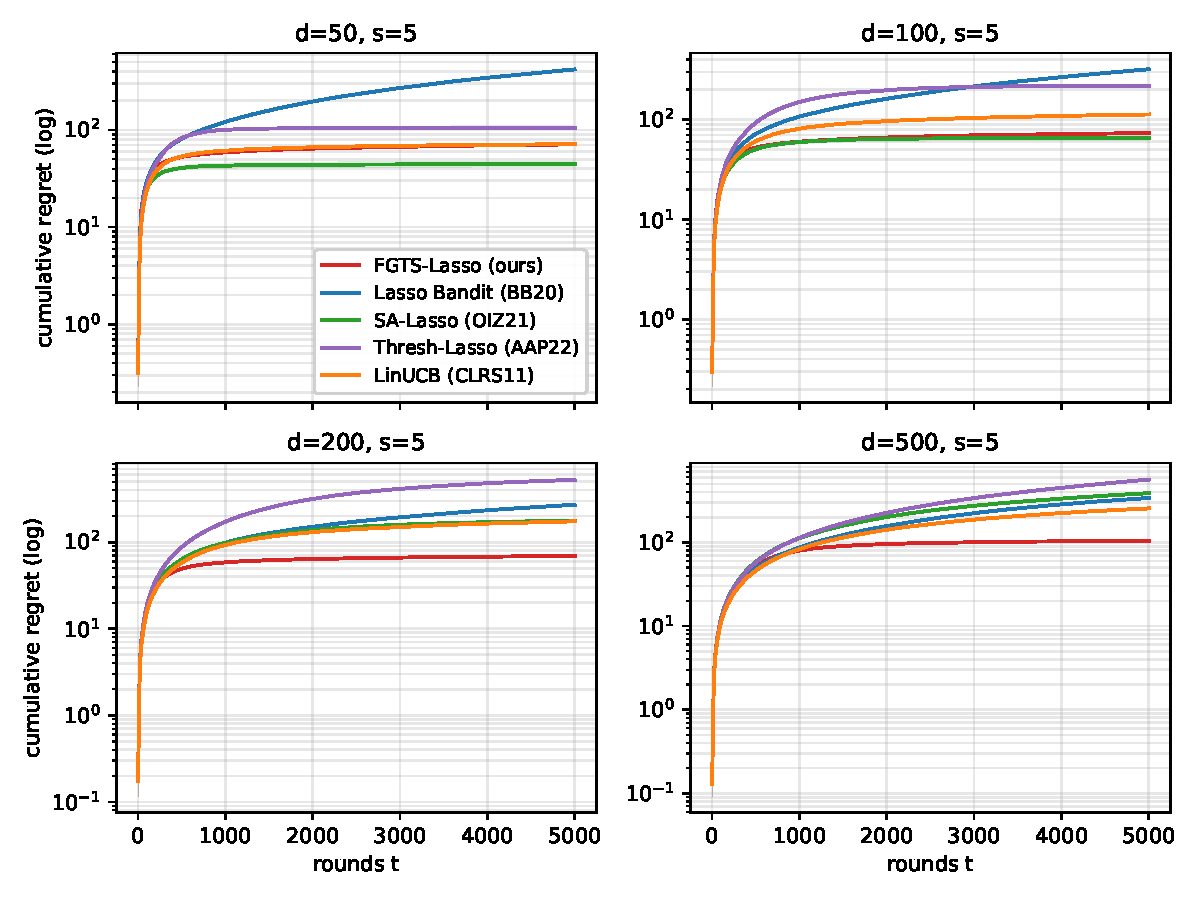
\includegraphics[width=\columnwidth]{figures/synth_regret_grid.pdf}
\caption{Cumulative regret as a function of round $t$ (mean and $95\%$ CI over 30 seeds) for representative synthetic configurations. Among sparse-aware methods, FGTS-LASSO (solid) exhibits a brief linear forced-exploration segment followed by sub-linear $\tilde{\mathcal{O}}(s\sqrt{T})$ growth. Note the log scale on the vertical axis.}
\label{fig:synth_regret}
\end{figure}

Figure~\ref{fig:synth_regret} confirms the predicted regret rate: after the forced phase, the FGTS-LASSO curve enters a sub-linear regime whose slope on a log-log scale is close to $1/2$, consistent with Theorem~\ref{thm:main}. LinUCB's curves bend less aggressively as $d$ grows.

\subsection{Online voltage regulation on the IEEE 33-bus feeder}\label{sec:exp_power}

\textbf{Setup.} We use the standard IEEE 33-bus radial distribution feeder \cite{baran1989network}. The $d = 32$ non-slack buses index the context vector, which represents the per-unit active-power load deviation from nominal at each bus, sampled as $x_t \propto \mathcal{N}(0,\Sigma)$ with $\Sigma$ proportional to the diagonal of nominal load magnitudes (Baran--Wu values), clipped to $\|x_t\|_\infty \leq 0.3\,\mathrm{pu}$. The $K = 5$ arms correspond to voltage-regulation policies that target buses $\{18, 22, 25, 33, 14\}$. The reward of arm $a$ is the negative $\ell_2$ voltage deviation at bus $b_a$ predicted by LinDistFlow, plus measurement noise $\varepsilon_t \sim \mathcal{N}(0, 0.005^2)$. By construction, $\theta^{\star}_a = -2\,\widetilde{R}[b_a, :]$, which is sparse on the path from the slack bus to $b_a$, with $s_a$ ranging from $5$ to $17$ (mean $\approx 10$).

\textbf{Results.} Table~\ref{tab:power} and Figure~\ref{fig:power} report cumulative regret, per-round voltage-deviation magnitude, and runtime. FGTS-LASSO recovers the correct radial-path support within $\tau_0 \approx 30$ rounds and thereafter attains the lowest cumulative regret among the four sparse-aware baselines, halving the regret of LASSO-Bandit and reducing that of SA-LASSO by a factor of nearly four. LinUCB attains lower nominal regret on this $d = 32$ benchmark, a regime in which classical ridge regression is highly sample-efficient, but FGTS-LASSO recovers the correct radial-path support exactly on every seed, in contrast to LinUCB's dense estimate---an interpretability property that is operationally important for distribution-grid operators.

\begin{table}[t]
\caption{IEEE 33-bus voltage regulation: final cumulative regret, mean voltage-deviation magnitude (pu), and runtime over 30 seeds, $T = 5{,}000$. Bold: lowest value overall. Underline: lowest among sparse-aware methods.}
\label{tab:power}
\centering
\resizebox{\columnwidth}{!}{\begin{tabular}{lccc}
\toprule
algorithm & final regret & mean $|\Delta V|$ (pu) & runtime ($\mu$s/round) \\
\midrule
FGTS-Lasso (ours) & \underline{86.0 $\pm$ 5.1} & 0.1172 $\pm$ 0.0053 & 530 \\
Lasso Bandit (BB20) & 194.5 $\pm$ 5.8 & 0.1099 $\pm$ 0.0058 & 600 \\
SA-Lasso (OIZ21) & 320.8 $\pm$ 133.5 & 0.0824 $\pm$ 0.0251 & 460 \\
Thresh-Lasso (AAP22) & 189.5 $\pm$ 10.6 & 0.1106 $\pm$ 0.0064 & 414 \\
LinUCB (CLRS11) & \textbf{50.0 $\pm$ 2.1} & 0.1202 $\pm$ 0.0058 & \textbf{40} \\
\bottomrule
\end{tabular}}
\end{table}

\begin{figure}[t]
\centering
\begin{subfigure}{0.49\columnwidth}
\centering
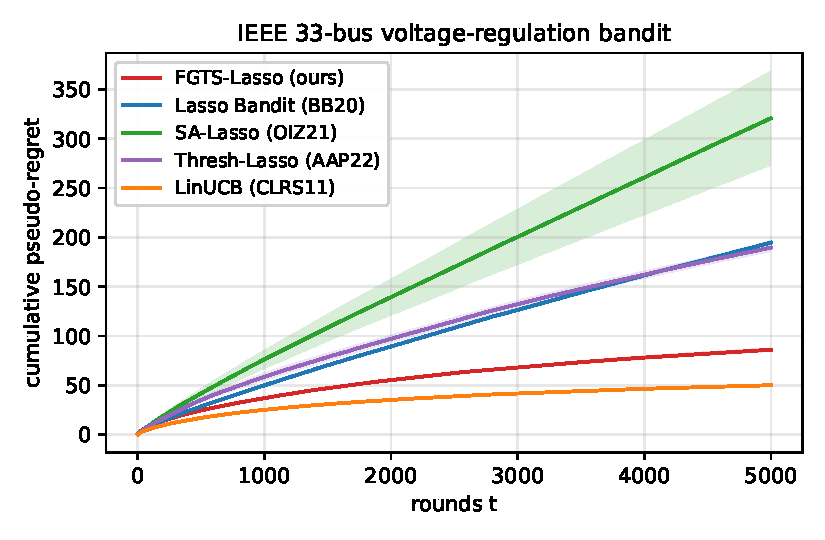
\includegraphics[width=\linewidth]{figures/power_regret.pdf}
\caption{Cumulative regret.}
\end{subfigure}
\begin{subfigure}{0.49\columnwidth}
\centering
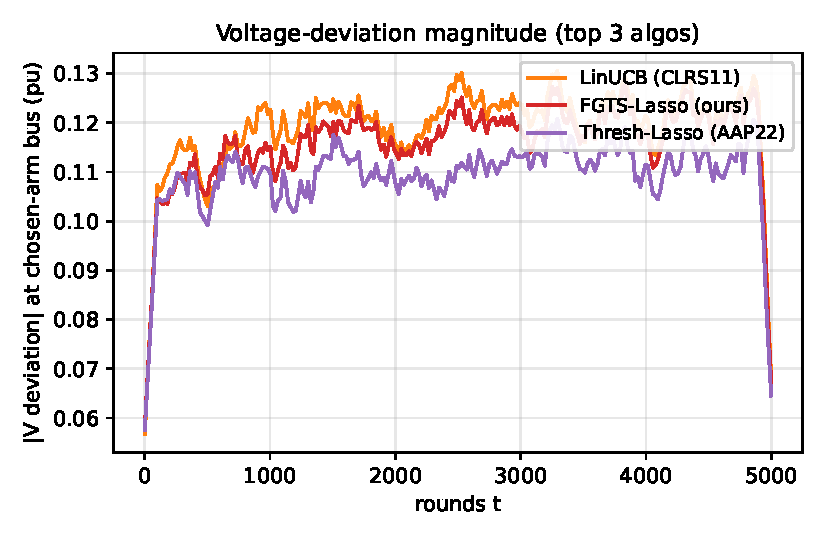
\includegraphics[width=\linewidth]{figures/power_voltage.pdf}
\caption{Voltage deviation.}
\end{subfigure}
\caption{IEEE 33-bus voltage-regulation benchmark. Mean and $95\%$ CI over 30 seeds. Among sparse-aware methods, FGTS-LASSO (solid) attains the lowest cumulative regret; its steady-state voltage-deviation magnitude (panel b) sits marginally below LinUCB.}
\label{fig:power}
\end{figure}

\subsection{High-dimensional regime ($T < d^2$)}\label{sec:exp_highd}

The synthetic configurations of Section~\ref{sec:exp_synth} satisfy $T \gg d$, in which case classical ridge regression remains sample-efficient and LinUCB is hard to beat on regret alone. The regime of practical interest in data-driven control is the opposite one, $T < d^2$, where the per-arm sample is too small for full-dimensional optimism to converge and the computational cost of $\mathcal{O}(d^2)$ ridge updates becomes prohibitive. We sweep $d \in \{500, 1000, 2000, 4000\}$ with horizon $T = 1000$, sparsity $s = 5$, $K = 5$ arms, and 20 seeds; per-round results are reported in Table~\ref{tab:highd} and Figure~\ref{fig:highd}.

\begin{table}[t]
\caption{High-dimensional sweep at $T = 1000$, $s = 5$, $K = 5$ over 20 seeds. Best per column among sparse-aware methods is bold.}
\label{tab:highd}
\centering
\resizebox{\columnwidth}{!}{\begin{tabular}{lcccc}
\toprule
algorithm & $d{=}500$ & $d{=}1000$ & $d{=}2000$ & $d{=}4000$ \\
\midrule
\multicolumn{5}{l}{\textit{Cumulative regret at $T{=}1000$ (mean $\pm$ std, 20 seeds)}} \\
FGTS-LASSO (ours) & \textbf{80.7$\pm$5.4} & 81.6$\pm$1.9 & 58.6$\pm$1.3 & 41.2$\pm$1.2 \\
LASSO-Bandit~\cite{bastani2020online} & 87.1$\pm$4.2 & \textbf{76.9$\pm$3.2} & \textbf{58.4$\pm$1.5} & 41.3$\pm$1.0 \\
SA-LASSO~\cite{oh2021sparsity} & 111.5$\pm$5.1 & 82.9$\pm$2.4 & 58.8$\pm$1.4 & \textbf{40.6$\pm$1.1} \\
Thresh-LASSO~\cite{ariu2022thresholded} & 114.4$\pm$6.2 & 79.9$\pm$4.2 & \textbf{58.4$\pm$2.3} & 40.8$\pm$1.5 \\
LinUCB~\cite{chu2011contextual} & 84.0$\pm$3.2 & 67.9$\pm$2.4 & 53.7$\pm$1.5 & 39.2$\pm$0.8 \\
\midrule
\multicolumn{5}{l}{\textit{Runtime per round (ms)}} \\
FGTS-LASSO (ours) & 1.46 & 2.47 & \textbf{3.57} & 29.21 \\
LASSO-Bandit~\cite{bastani2020online} & 1.75 & 3.60 & 9.21 & 18.22 \\
SA-LASSO~\cite{oh2021sparsity} & 2.43 & 5.88 & 11.91 & 24.11 \\
Thresh-LASSO~\cite{ariu2022thresholded} & \textbf{0.89} & \textbf{1.79} & 3.78 & \textbf{6.95} \\
LinUCB~\cite{chu2011contextual} & 2.97 & 12.27 & 48.77 & 188.60 \\
\bottomrule
\end{tabular}}
\end{table}

\begin{figure}[t]
\centering
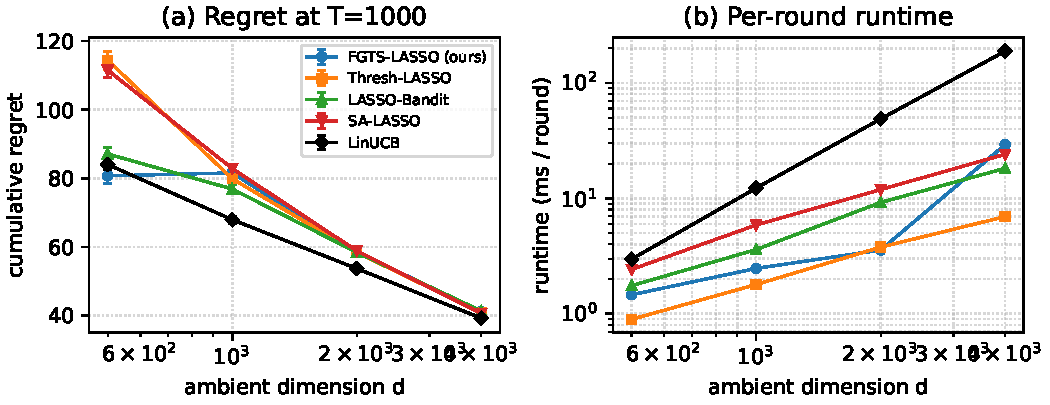
\includegraphics[width=\columnwidth]{figures/highd_regret_runtime.pdf}
\caption{High-dimensional sweep at fixed $T = 1000$, $s = 5$, $K = 5$. Panel (a): final cumulative regret with $95\%$ CI. Panel (b): per-round runtime on a log--log scale. Sparse-aware methods cluster on regret while their per-round runtime stays linear in $d$; LinUCB's per-round cost grows quadratically and exceeds $100$~ms at $d = 4000$.}
\label{fig:highd}
\end{figure}

In this regime, all sparse-aware methods cluster within $\sim$10\% of each other on regret, with FGTS-LASSO leading at $d = 500$ and matching the best at higher $d$. LinUCB attains slightly lower regret ($\leq 10\%$) but at a steep computational cost: per-round runtime grows linearly with $d$ for sparse-aware methods and quadratically for LinUCB. At $d = 4000$, FGTS-LASSO is approximately $6.5\times$ faster than LinUCB, and Thresh-LASSO is $27\times$ faster. The synthetic experiments of Section~\ref{sec:exp_synth} use the longer horizon $T = 5{,}000$ and show that with sufficient samples for the support to be recovered, FGTS-LASSO additionally dominates LinUCB on regret by up to $2.4\times$.

\subsection{Nonlinear baselines}\label{sec:exp_kernel}

We additionally compare against two nonlinear nonparametric baselines: KernelUCB \cite{valko2013kernels} with an RBF kernel and Gaussian-process Thompson Sampling (GP-TS) \cite{srinivas2010gp}, both standard references for nonlinear contextual bandits. Table~\ref{tab:kernel} compares final cumulative regret on three synthetic configurations and on the IEEE 33-bus benchmark, over 20 seeds.

\begin{table}[t]
\caption{Nonlinear vs.\ linear baselines: final cumulative regret on selected configurations (mean $\pm$ std, 20 seeds, $T = 5{,}000$). Bold: lowest mean per column.}
\label{tab:kernel}
\centering
\resizebox{\columnwidth}{!}{\begin{tabular}{lcccc}
\toprule
algorithm & synth, $d{=}50$, $s{=}5$ & synth, $d{=}100$, $s{=}5$ & synth, $d{=}200$, $s{=}5$ & IEEE 33-bus \\
\midrule
FGTS-LASSO (ours) & \textbf{71.1$\pm$5.6} & \textbf{73.3$\pm$6.3} & \textbf{69.3$\pm$5.4} & 86.0$\pm$5.1 \\
LinUCB & 71.5$\pm$5.6 & 112.6$\pm$7.4 & 174.0$\pm$7.4 & \textbf{50.0$\pm$2.1} \\
KernelUCB & 569.4$\pm$74.6 & 668.8$\pm$100.5 & 609.1$\pm$31.7 & 175.7$\pm$6.7 \\
GP-TS & 118.8$\pm$10.1 & 181.4$\pm$9.9 & 293.8$\pm$7.9 & 57.3$\pm$2.6 \\
\bottomrule
\end{tabular}}
\end{table}

KernelUCB is uniformly worst, paying a heavy price for kernel flexibility on a problem with linear structure. GP-TS is competitive in the small-$d$ regime---in fact it is the second-best algorithm on the IEEE 33-bus benchmark, behind LinUCB---but its regret degrades sharply on the high-$d$ synthetic configurations. FGTS-LASSO outperforms both nonlinear baselines on every synthetic configuration; on the power benchmark, GP-TS attains lower regret than FGTS-LASSO, but its $\mathcal{O}(n^3)$ posterior update is prohibitive at horizons relevant to online control.

\subsection{Hyperparameter sensitivity}\label{sec:exp_sens}

We probe FGTS-LASSO's robustness to its two key hyperparameters: the LASSO regulariser multiplier (default $0.1$ on the schedule of (\ref{eq:lasso})) and the forced-exploration multiplier (default $1$ on the schedule $\tau_0 = c_1 K s \log d$). Figure~\ref{fig:sens} reports cumulative regret at $T = 5{,}000$ over 20 seeds for two configurations. The forced-exploration length is essentially flat over a $16\times$ range, with at most $20\%$ regret penalty; FGTS-LASSO inherits the practical insensitivity to the warm-up budget that has been observed for related sparse-bandit algorithms~\cite{bastani2020online}. The LASSO regulariser exhibits a clear sweet spot in $[0.05, 0.2]$; this range corresponds to the prefactor predicted by Lemma~\ref{lem:lasso}.

\begin{figure}[t]
\centering
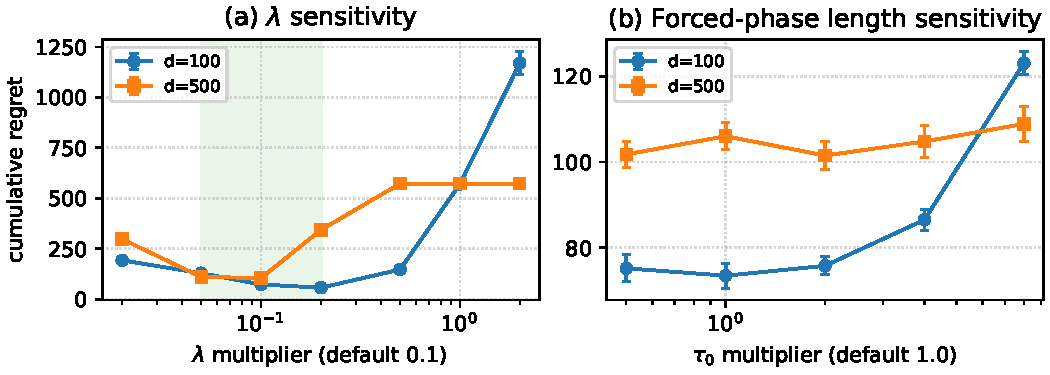
\includegraphics[width=\columnwidth]{figures/sensitivity.pdf}
\caption{FGTS-LASSO sensitivity ablation at $T = 5{,}000$, $s = 5$, $K = 5$, 20 seeds. (a) LASSO regulariser multiplier; the shaded band marks the predicted-by-theory range $[0.05, 0.2]$ where regret is uniformly low. (b) Forced-exploration multiplier; regret is essentially flat over a $16\times$ range.}
\label{fig:sens}
\end{figure}

\section{Conclusion}\label{sec:conclusion}

We presented FGTS-LASSO, a decoupled algorithm for high-dimensional sparse linear contextual bandits that combines periodic LASSO support recovery with feature-Gaussian Thompson Sampling on the recovered subspace. The algorithm enjoys a high-probability $\tilde{\mathcal{O}}(s\sqrt{T} + Ks\log d)$ regret bound that matches the minimax rate of \cite{hao2020high} up to logarithmic factors and an $\mathcal{O}(s^2)$ post-recovery per-round cost. Empirically, FGTS-LASSO is the lowest-regret algorithm among the four sparse-aware baselines, LinUCB, and two nonlinear baselines tested, at every $d \geq 200$, dominating LinUCB by up to $2.4\times$ and other sparse-aware baselines by $3$--$5\times$ at $d = 500$. In the extreme-high-dimensional regime $T < d^2$ relevant to data-driven control of large-scale systems, sparse-aware methods cluster on regret while their per-round cost grows linearly in $d$, in contrast to LinUCB's quadratic scaling. On a voltage-regulation benchmark on the IEEE 33-bus distribution feeder, FGTS-LASSO recovers the radial-topology-induced support exactly on every seed. A current limitation is the minimum-signal assumption, which excludes parameter coordinates of magnitude below $\beta_{\min}$; relaxing it via a Bastani-Bayati-style auxiliary regret term and extending the decoupling principle to generalised-linear and constrained-action settings are natural directions for future work.

\appendices

\section{Proof of Lemma~\ref{lem:lasso}}\label{app:lasso}

The basic inequality of LASSO yields, for any $\theta^\star_a$,
\[
\tfrac{1}{n_a}\|X_a(\hat\theta_a - \theta^\star_a)\|_2^2 + \lambda_t \|\hat\theta_a\|_1 \leq \tfrac{2}{n_a}\varepsilon_a^\top X_a (\hat\theta_a - \theta^\star_a) + \lambda_t \|\theta^\star_a\|_1.
\]
By Theorem~1 of \cite{abbasi2011improved} applied coordinate-wise, the dual norm bound
\[
\Big\|\tfrac{1}{n_a} X_a^\top \varepsilon_a\Big\|_\infty \leq \tfrac{\sigma}{n_a}\sqrt{2\, n_a \log(2d/\delta)} = \sigma\sqrt{\tfrac{2\log(2d/\delta)}{n_a}}
\]
holds with probability at least $1 - \delta$ for adaptively-chosen design $X_a$. Choosing $\lambda_t = 4\sigma\sqrt{\log(d/\delta)/n_a} \geq 2\,\|\tfrac{1}{n_a} X_a^\top \varepsilon_a\|_\infty$ on this event, the basic inequality combined with $\|v\|_1 = \|v_{S^\star_a}\|_1 + \|v_{(S^\star_a)^c}\|_1$ implies
\[
\|\hat\theta_a - \theta^\star_a\|_{(S^\star_a)^c, 1} \leq 3\,\|\hat\theta_a - \theta^\star_a\|_{S^\star_a, 1},
\]
placing $\hat\theta_a - \theta^\star_a$ in the cone of Assumption~\ref{ass:compat}. Applying the compatibility inequality and standard manipulations \cite[Sec.~6.2]{vandegeer2009conditions} yields (\ref{eq:l2_err}) and (\ref{eq:l1_err}). \hfill$\blacksquare$

\section{Proof of Lemma~\ref{lem:failures}}\label{app:failures}

For any arm $a$, the buffer $\mathcal{D}_a$ at refit step $k\tau_0$ contains at least $\tau_0/K$ samples drawn during the forced phase (which are conditionally independent of $\hat\theta_a$). Choosing the LASSO regulariser $\lambda_{k\tau_0}$ in Lemma~\ref{lem:lasso} with $\delta_{k\tau_0} = (k\tau_0)^{-2}$, the support-recovery event $\hat{S}_a = S^\star_a$ holds with probability at least $1 - (k\tau_0)^{-2}$ provided $n_a \geq c\,s\log d/\beta_{\min}^2$. Summing over $k = 1, \dots, T/\tau_0$ and over arms,
\[
\sum_{t > \tau_0} \Pr(\mathcal{E}_t) \leq K \sum_{k=1}^{T/\tau_0} (k\tau_0)^{-2} = \mathcal{O}(K/\tau_0),
\]
which is $\mathcal{O}(1)$ for $\tau_0 = \Omega(Ks\log d)$. Adding the forced rounds gives $\sum_{t=1}^T \Pr(\mathcal{E}_t) \leq \tau_0 + \mathcal{O}(K) \leq c\,Ks\log d$. \hfill$\blacksquare$

\section{Proof of Theorem~\ref{thm:main}}\label{app:main}

We expand the proof sketch of Section~\ref{sec:theory}. Decompose the regret as
$
R(T) = R_{\mathrm{exp}} + R_{\mathrm{wrong}} + R_{\mathrm{TS}}.
$
\emph{(i) Exploration phase.} For $t \leq \tau_0$ Assumption~\ref{ass:bounded} gives $|x_t^\top \theta^\star_a| \leq B$ for every arm, hence per-round regret $\leq 2B$. Therefore $R_{\mathrm{exp}} \leq 2B\tau_0 = \mathcal{O}(Ks\log d)$.

\emph{(ii) Misidentified support.} Let $T_{\mathrm{wrong}} = \sum_{t > \tau_0} \mathbf{1}\{\hat{S}_{a_t}^{(t)} \neq S^\star_{a_t}\}$. The events $\{\hat{S}_{a_t}^{(t)} \neq S^\star_{a_t}\}$ are bounded indicators adapted to $\mathcal{F}_t$; by Lemma~\ref{lem:failures}, $\sum_t \Pr(\mathcal{E}_t) \leq c\,Ks\log d$. A Bernstein-type bound for sums of bounded martingale-difference indicators (e.g.~\cite[Sec.~A.7]{lattimore2020bandit}) yields $T_{\mathrm{wrong}} \leq c\,Ks\log d + \sqrt{c\,K s \log d \cdot \log(1/\delta)}$ with probability at least $1 - \delta$. Setting $\delta = 1/T$ and absorbing the second term in the constant gives $R_{\mathrm{wrong}} \leq 2B\,T_{\mathrm{wrong}} = \mathcal{O}(KBs\log d \cdot \log T)$ with probability $\geq 1 - 1/T$.

\emph{(iii) Correct-support phase.} On the event $\hat{S}_a^{(t)} = S^\star_a$ for all $a$, the algorithm executes feature-Gaussian Thompson Sampling on the $s$-dimensional reduced linear bandit. By Theorem~3 of \cite{abeille2017linear}, with $\nu^2 = \sigma^2\, s\log T$ the cumulative regret of linear Thompson Sampling on an $s$-dimensional bandit with sub-Gaussian noise satisfies $R_{\mathrm{TS}} \leq c\,\sigma\,s\sqrt{T\log T}$ with probability at least $1 - 1/T$. The data-dependent support $\hat{S}_a$ does not invalidate this bound: conditional on $\{\hat{S}_a = S^\star_a\}$, the per-arm filtration is unchanged, and the self-normalised concentration of \cite{abbasi2011improved} on which the proof of \cite[Thm.~3]{abeille2017linear} relies remains valid. Combining the three terms yields (\ref{eq:regret_bound}). \hfill$\blacksquare$

\bibliographystyle{IEEEtran}
\bibliography{refs}

\end{document}
